\documentclass{iagtese} 		% declara��o da classe iagtese com
						% padr�es de formata��o.
						%	
%\documentclass{iagtese_en}	% declara��o da classe iagtese em
						% ingles. Para escrever a tese em 
						% ingles, descomente esta linha e 
						% comente a linha anterior.
						%				%	
%\hypercolor				% links coloridos para a versao
						% on line da tese. Para usar esta
						% opcao descomente esta linha.
						% 	
\begin{document}			% in�cio do documento
						% 				
\institution{Universidade de S�o Paulo \\ Instituto de Astronomia, Geof�sica e Ci�ncias Atmosf�ricas \\ Departamento de Astronomia}

\title{T�tulo do trabalho}

\translator{{Tese/Disserta��o apresentada ao Departamento de Astronomia do Instituto de Astronomia, Geof�sica e Ci�ncias Atmosf�ricas da Universidade de S�o Paulo como requisito parcial para a obten��o do t�tulo de Mestre/{}Doutor em Ci�ncias.\\ \\
�rea de Concentra��o: Astronomia\\
Orientador(a): Prof.($^{\rm a}$) Dr.($^{\rm a}$) Orientador(a)}}

\author{Autor}

\date{S�o Paulo \ano}
			% arquivo para inserir a capa
						%
\pagestyle{empty}			% padr�o de formata��o para parte
						% inicial do texto
						%
\maketitle					% 
						%
\Dedicatoria				%
\hfill
\vfill
\hfill{\it{sua dedicatoria aqui!}}
\vspace{2cm}


		%
						% componentes iniciais do trabalho
\Agradecimentos			%
� minha fam�lia;

� fulana;

� orientadora;

Aos pesquisadores;

� Professora;

Aos colegas: 1, 2, 3 e 4

� FAPESP, pelo apoio financeiro, sob o projeto n$^o$: 6666/6666;

�s Institui��es

\vfill

\begin{flushleft}
\rule{6cm}{0.5pt}\\
{\footnotesize{Esta tese/disserta��o foi escrita em \LaTeX{} com a classe IAGTESE, para teses e disserta��es do IAG.}}
\end{flushleft}
	% caso n�o queira adicionar algum
						% deles, simplesmente remova as
						% linhas correspondentes.
						%
\Epigrafe					%  
\vfill
\begin{flushright}

``\textit{frase bonita 01}''\\

\vspace{0.4cm}

Autor da frase bonita 01

\end{flushright}

\vspace{0.5cm}

\begin{flushright}

``\textit{frase bonita 02}''\\

\vspace{0.4cm}

Autor da frase bonita 02

\end{flushright}

\vspace{2cm}
		%
						%
\Resumo					%
% Autor: Gabriel Góes Rocha de Lima
% Descrição: Resumo do postesr para o II workshop Inteligência Artificial e Geociências

\documentclass[11pt]{article} % declaração do tipo de documento
\usepackage[utf8]{inputenc} % declaração do tipo de codificação
\usepackage{geometry} % pacote para definição de margens
\usepackage{ragged2e} % Texto justificado
\usepackage{indentfirst} % pacote para indentação do primeiro parágrafo
\usepackage{setspace} % pacote para definição de espaçamento
\usepackage{titlesec} % Pacote para formatação de títulos

\geometry{a4paper, left=2cm, right=2cm, top=2cm, bottom=2cm} % definição das margens
\onehalfspacing % espaçamento de 1.5
\setlength{\parindent}{1.25cm} % indentação de 1.25cm
\setlength{\parskip}{0.5em} % set distance spacing between paragraphs
%\renewcommand{\baselinestretch}{1.5} % set line spacing
%\setmainfont{SourceCodePro Nerd Font} % Definindo a fonte principal
\titleformat{\section}{\normalfont\bfseries}{\thesection}{1em}{} % Formatação de títulos de seção
\titleformat{\subsection}{\normalfont\bfseries}{\thesubsection}{1em}{} % Formatação de títulos de subseção


\begin{document} % início do documento
\title{Da Terra ao Código: Integrando Dados Geológicos com Inteligência Computacional} % título do documento
\author{Gabriel Góes Rocha de Lima} % autor do documento
\date{28 de fevereiro de 2024} % data do documento
\maketitle % criação do título

% Transformar texto em itálico
\newcommand{\italic}[1]{\textit{#1}}

\par{
Este projeto propõe a criação de uma abordagem integrada que combina bases de dados
geológicas a modelos de classificação litológica, visando avançar nas
metodologias de exploração mineral. Em fase conceitual, esta iniciativa busca estabelecer
uma colaboração multidisciplinar entre geocientistas e programadores, visando
desenvolver uma plataforma que permita a geração e atualização dinâmica de mapas
litológicos preditivos. Central para este empreendimento é o desenvolvimento de um
sistema que, ao integrar dados geológicos precisos com algoritmos de aprendizado de
máquina, possibilite a criação de mapas com uma acurácia aprimorada ao longo do tempo.
Este processo iterativo de aperfeiçoamento se baseia na inclusão contínua de novos dados
e na avaliação rigorosa de métricas de desempenho, tais como precisão, sensibilidade
(\italic{recall}), e valor F1, além da análise da área sob a curva ROC. Estas métricas são vitais
para assegurar a confiabilidade e aplicabilidade das classificações do sistema no campo
da exploração mineral. A infraestrutura tecnológica proposta para sustentar tal sistema
envolve a utilização do PostgreSQL e da extensão PostGIS, criando um fundamento sólido
para o gerenciamento e análise eficientes de dados geoespaciais. Essa configuração não
apenas suportará as análises complexas requeridas pelo projeto mas também permitirá
uma gestão dinâmica e sistemática dos dados. Além disso, a implementação de folhas
cartográficas no processo de mapeamento assegurará que o sistema seja capaz de
adaptar-se a uma ampla gama de contextos geológicos, melhorando a classificação de
litologias e identificação de locais com potencial de mineralização. Adicionalmente, o
projeto aspira expandir suas capacidades para incluir a geração de mapas prospectivos
minerais preditivos. Este avanço significativo tem o potencial de transformar a exploração
mineral, indicando áreas com elevado potencial de mineralização e, consequentemente,
promovendo uma exploração mais eficiente e direcionada. Ao apresentar esta proposta
inovadora no \italic{II Workshop Intelli+Geo}, visa-se não apenas fomentar um debate
enriquecedor sobre as fronteiras entre geociências e tecnologia da informação, mas
também demonstrar a viabilidade e o potencial impactante do conceito através de um
esboço de protótipo funcional. Este protótipo inicial, ainda em estágios rudimentares de
desenvolvimento, serve como prova de conceito, ilustrando a capacidade de integração de
dados geológicos e modelos de classificação para aprimorar a precisão e eficácia na
exploração mineral. A partilha desta fase preliminar com especialistas e acadêmicos do
setor procura não apenas validar a abordagem proposta, mas também angariar
colaborações estratégicas e \italic{insights} valiosos que contribuam para a evolução do projeto.
}


\end{document} % fim do documento

		%
						%
\Abstract					%
\input{tex/abstract.tex}		%
						%
\listoffigures 				% lista de figuras (opcional)
\listoftables 				% lista de tabelas (opcional)
\tableofcontents 			% sum�rio
						%
\cleardoublepage			%
\pagestyle{fancy}			% formata��o para corpo do texto
						%
\chapter{Introdu��o}
\label{intro}

\section{como incluir cita��es utilizando bibTeX}

\begin{verbatim}O comando \citet{doutorado} produz:\end{verbatim}
\citet{doutorado}

\begin{verbatim}O comando \citet{mestrado} produz:\end{verbatim}
\citet{mestrado}

\begin{verbatim}O comando \citet*{artigo1} produz:\end{verbatim}
\citet*{artigo1}

\begin{verbatim}O comando \citet{artigo2} produz:\end{verbatim}
\citet{artigo2}

\begin{verbatim}O comando \citet{bethe} produz:\end{verbatim}
\citet{bethe}

\begin{verbatim}O comando \citet{livro} produz:\end{verbatim}
\citet{livro}

\begin{verbatim}O comando \citet{feynman} produz:\end{verbatim}
\citet{feynman}

\begin{verbatim}O comando \cite{salpeter} produz:\end{verbatim}
\cite{salpeter}

\section{pr�xima se��o}

\subsection{subse��o}

\subsubsection{subsubse��o}

\paragraph{par�grafo}
		%
\chapter{Base de dados}\label{database}

Base de dados. Citar figura \ref{identificador}.

\begin{figure}[!ht]
\begin{center}
\setcaptionmargin{1cm}
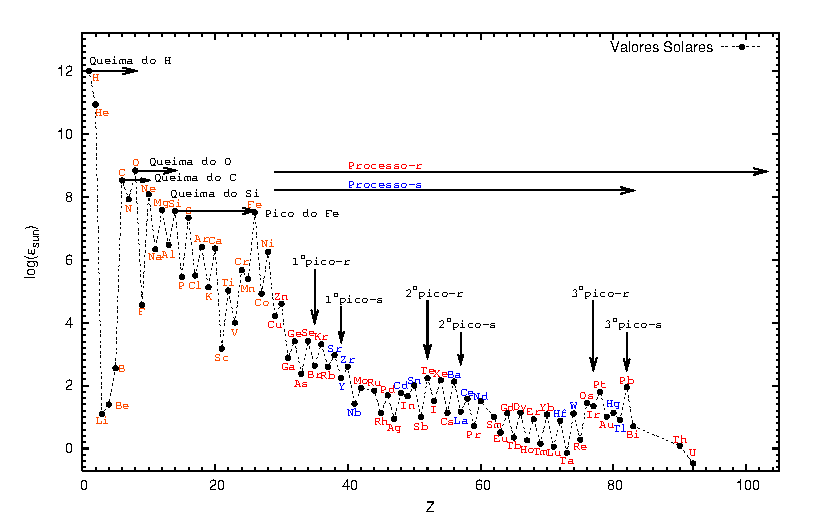
\includegraphics[width=1.0 \columnwidth,angle=0]{fig/solar_grevesse.eps}
\caption[Resumo da legenda da figura (aparece na lista de figuras)]{Legenda da figura.} 
\label{identificador}
\end{center}
\end{figure}


\begin{center}
\setcaptionmargin{1cm}
\scriptsize
\begin{longtable}{lcccc}
\caption[Resumo da legenda da tabela (aparece na lista de figuras)]{Exemplo de tabela feita com o longtable.}\\
\hline \hline \\[-2ex]
\multicolumn{1}{c}{Coluna1} &
\multicolumn{1}{c}{Coluna2} &
\multicolumn{1}{c}{Coluna3} &
\multicolumn{1}{c}{Coluna4} &
\multicolumn{1}{c}{Coluna5} 

\\[0.5ex] \hline
\\[-1.8ex]

\endfirsthead

\multicolumn{5}{c}{\footnotesize{{\slshape{{\tablename} \thetable{}}} - Continua��o}}\\[0.5ex]

\hline \hline\\[-2ex]

\multicolumn{1}{c}{Coluna1} &
\multicolumn{1}{c}{Coluna2} &
\multicolumn{1}{c}{Coluna3} &
\multicolumn{1}{c}{Coluna4} &
\multicolumn{1}{c}{Coluna5} 

\\[0.5ex] \hline
\\[-1.8ex]

\endhead

\multicolumn{3}{l}{{\footnotesize{Continua na pr�xima p�gina\ldots}}}\\
\endfoot
\hline

\endlastfoot

1 & 2 & 3 & 4 & 5 \\
6 & 7 & 8 & 9 & 10\\

\label{tabela_com_longtable}
\end{longtable}
\end{center}


    	% inserir os cap�tulos do seu
\input{tex/analise.tex}		% trabalho.
% Conclusão
\setlength{\fboxsep}{1cm}% Espaçamento interno do fbox
\fbox{% Cria um box ao redor do texto
    \parbox{\textwidth}{% Permite o controle de parágrafo dentro do fbox
        \setlength{\parindent}{1.5cm} % Define a identação dos parágrafos
        \fontsize{30}{36}\selectfont % Ajusta o tamanho da fonte e o espaçamento de linha
        \textbf{Conclusão}\\

\par{
    O desenvolvimento deste projeto evidencia a importância da sinergia entre dados geológicos e inteligência artificial, apresentando um protótipo promissor que aguarda validação em ambientes de supercomputação. Esperamos que a divulgação desta iniciativa inspire a colaboração, não apenas para refinamento e ampliação do modelo existente, mas também para explorar seu pleno potencial em análises preditivas avançadas de mapeamento geológico. 
}\\

} % Fecha o parbox
} % Fecha o fbox
		% 
       						%
						%
%\begin{thebibliography}{99}	% refer�ncias bibliogr�ficas (d�
%\bibitem{Quireza et al. 2007}{quireza}Quireza C., Rocha-Pinto H. J., Maciel W. J., 2007, A\&A, 475, 217

\bibitem[Aoki et al.(2001)]{2001ApJ...561..346A} Aoki, W., Ryan, S. G., Norris, J. E., Beers, T. C., Ando, H., Iwamoto, N., Kajino, T., Mathews, G. J., \& Fujimoto, M. Y. 2001, ApJ 561, 346

\bibitem[Aoki et al.(2002)]{2002ApJ...580.1149A} Aoki, W., Ryan, S. G., Norris, J. E., Beers, T. C., Ando, H., \& Tsangarides, S. 2002, ApJ 580, 1149 

\bibitem[Wasserburg et al. (1994)]{1994ApJ...424..412W} Wasserburg, G. J., Busso, M., Gallino, R., \& Raiteri, C. M. 1994, ApJ 424, 412
 	% prefer�ncia ao bibTeX).
%\end{thebibliography}		% caso n�o use o bibTeX, remova os
						% comentarios das tr�s linhas
						% e comente a linha \bibliography
						%
\bibliography{tex/bibliografia}	% bibliografia utilizando bibTeX,
						% referente ao arquivo
						% bibliografia.bib na pasta tex/
						%
\begin{apendice}			% inicio do ambiente apendice
\chapter{t�tulo do ap�ndice 01}\label{ap01}

\section{subt�tulo 01}\label{subap01}

\chapter{t�tulo do ap�ndice 02}\label{ap02}
		% texto referente ao apendice
\end{apendice}				% fim do ambiente apendice. caso
						% nao utilize apendice, remova as
						% 3 linhas de comando.
						%
\end{document}				% fim do arquivo
